\chapter{2-D Convolutional Nerual Networks}
\label{3.2D_CNN}
\lhead{\emph{2-D Convolutional Neural Networks}}

During the development of the project, we have worked with four different PyEDDL versions (0.12, 0.13, 0.14 and 1.0.0) since this is a library currently in development. 3-D Convolutional Neural Networks were finally supported in PyEDDL version 1.0.0, which was released on May 27th 2021. Therefore the first CNN had to be 2-dimensionals.

This has two main drawbacks. The first one is the loss of some context information since our CNN can not analize at once a whole region of the MRI but it has to slice it, an issue inherent of working in a lower dimension. The second one is the need of having to consider also the different axles and orientations, which can be solved with data preprocessing.

\section{Data preprocessing}

For the 2-D CNN we have only used \textit{FLAIR} modality of the MRI. We first resize the \textit{FLAIR} image to $(256\times256\times256)$ so that, independently of the scanner used, the input has the same shape. After this we slice the data by the last axis. We decided this shape even when the first axis is being upsampled in all the MRI because it allows us to change the orientation or slicing axis and still having the same input shape so transfer learning techniques are possible. As a final preprocessing step we normalize each image.

No data augmentation techniques have been used since the final purpose of this project is not achieving the best accuracy (we remit to MICCAI 2016 challenge and later research works for that) but having a fair analysis and comparison of EDDL library.


%%%%%%% U-NET
\newpage
\section{U-Net}

U-Net \cite{UNET:2015} first appeared in 2015 and it quickly became the standard for biomedical image segmentation. We chose it as the model for our first approach. The network structure can be seen in the image below, the only change in the network structure in our implementation with respect to the one originally presented is that we have added batch normalization after each convolution for a better convergence and stability.

\begin{center}
\hspace*{15pt}
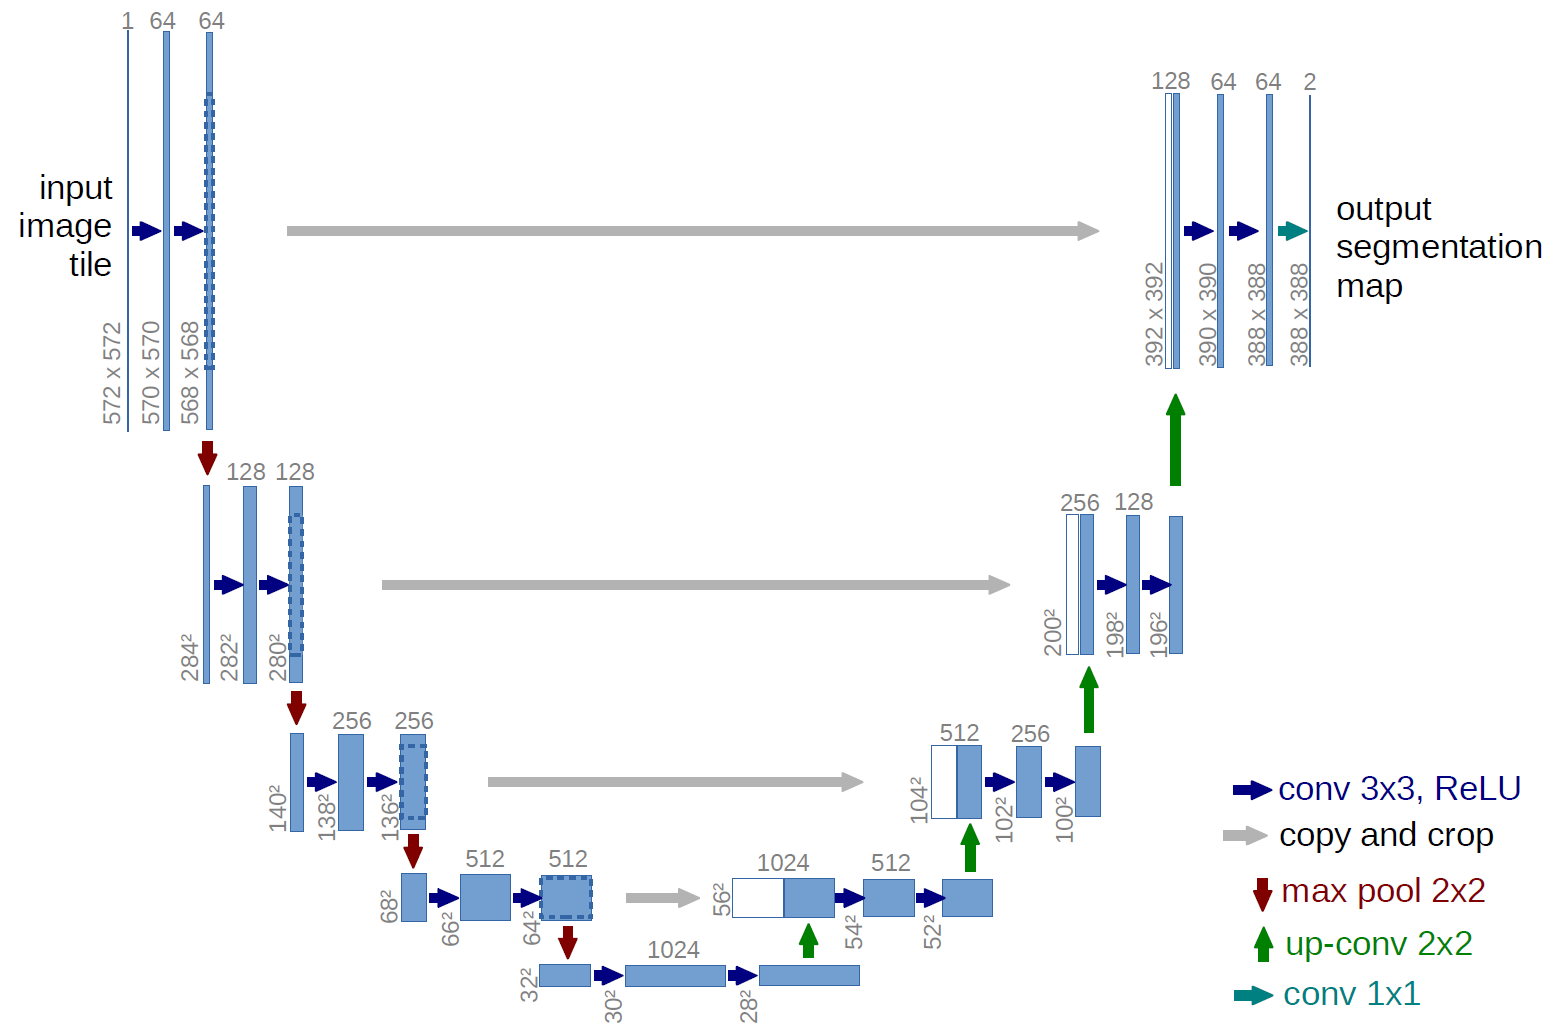
\includegraphics[width=\textwidth]{images/unet.png}
\captionof{figure}{U-Net model \cite{UNET:2015}}
\end{center}

% TODO: Ugly!
The training configuration was the following:
\begin{itemize}
    \item \textbf{Loss function: } Binary cross entropy.
    \item \textbf{Optimizer: } Adam, learning rate 0.0001
    \item \textbf{Batch size: } 8
\end{itemize}

\newpage
\subsection{U-Net evaluation}

% TODO: Loss function per epoch
% TODO: Dice metric per epoch
% TODO: Best accuracy acchieved

\begin{figure*}[!htb]
    \subfigure[tr943]{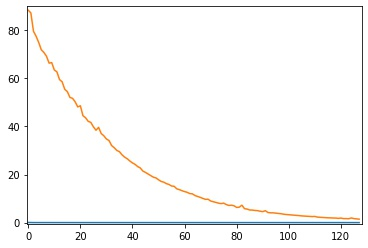
\includegraphics[width=.47\textwidth]{images/aux.jpg}\label{fig:tr943}}\hfill
    \subfigure[tr1426]{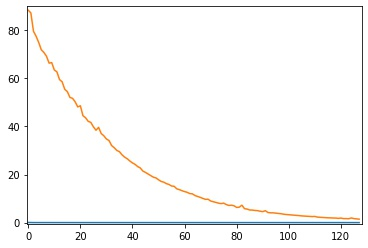
\includegraphics[width=.47\textwidth]{images/aux.jpg}\label{fig:tr1426}}
    
    \subfigure[tr943]{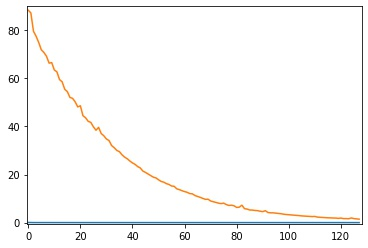
\includegraphics[width=.47\textwidth]{images/aux.jpg}\label{fig:tr943}}\hfill
    \subfigure[tr1426]{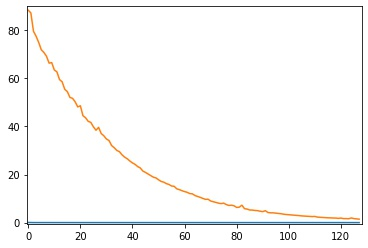
\includegraphics[width=.47\textwidth]{images/aux.jpg}\label{fig:tr1426}}
    
    \subfigure[tr943]{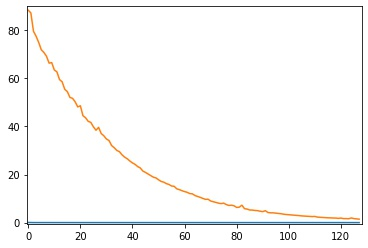
\includegraphics[width=.47\textwidth]{images/aux.jpg}\label{fig:tr943}}\hfill
    \subfigure[tr1426]{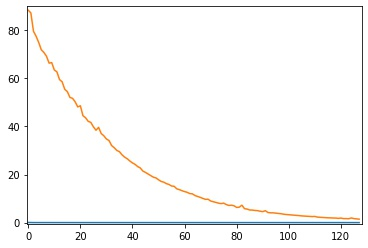
\includegraphics[width=.47\textwidth]{images/aux.jpg}\label{fig:tr1426}}

    \subfigure[tr943]{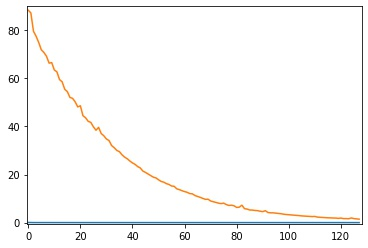
\includegraphics[width=.47\textwidth]{images/aux.jpg}\label{fig:tr943}}\hfill
    \subfigure[tr1426]{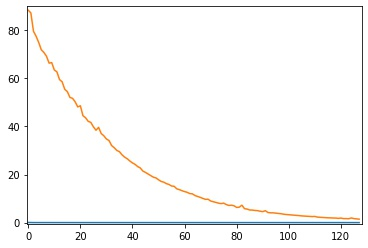
\includegraphics[width=.47\textwidth]{images/aux.jpg}\label{fig:tr1426}}
\end{figure*}


\newpage
\subsection{U-Net profiling}

\begin{figure*}[!htb]
    \subfigure[tr943]{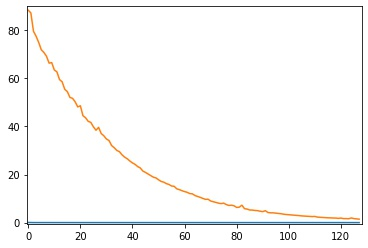
\includegraphics[width=.47\textwidth]{images/aux.jpg}\label{fig:tr943}}\hfill
    \subfigure[tr1426]{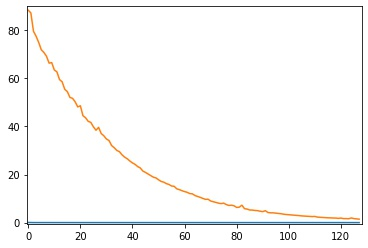
\includegraphics[width=.47\textwidth]{images/aux.jpg}\label{fig:tr1426}}
    
    \subfigure[tr943]{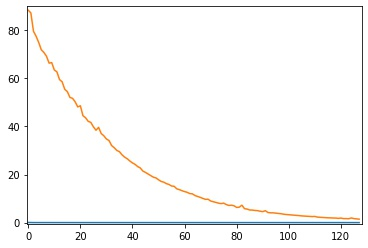
\includegraphics[width=.47\textwidth]{images/aux.jpg}\label{fig:tr943}}\hfill
    \subfigure[tr1426]{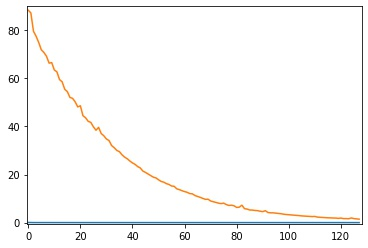
\includegraphics[width=.47\textwidth]{images/aux.jpg}\label{fig:tr1426}}
    
    \subfigure[tr943]{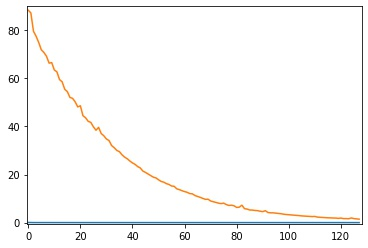
\includegraphics[width=.47\textwidth]{images/aux.jpg}\label{fig:tr943}}\hfill
    \subfigure[tr1426]{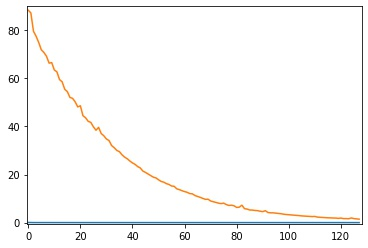
\includegraphics[width=.47\textwidth]{images/aux.jpg}\label{fig:tr1426}}

    \subfigure[tr943]{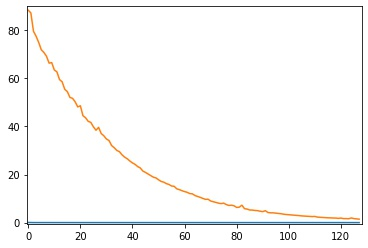
\includegraphics[width=.47\textwidth]{images/aux.jpg}\label{fig:tr943}}\hfill
    \subfigure[tr1426]{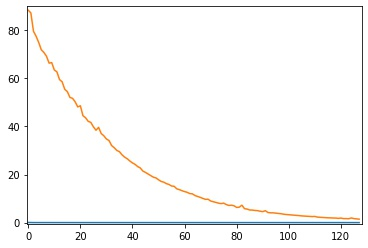
\includegraphics[width=.47\textwidth]{images/aux.jpg}\label{fig:tr1426}}
\end{figure*}



%%%%%%% DOUBLE U-NET
\newpage
\section{Double U-Net}
Start writing about Double U-Net.

% TODO: Describe the model
% TODO: Training parameters

\begin{center}
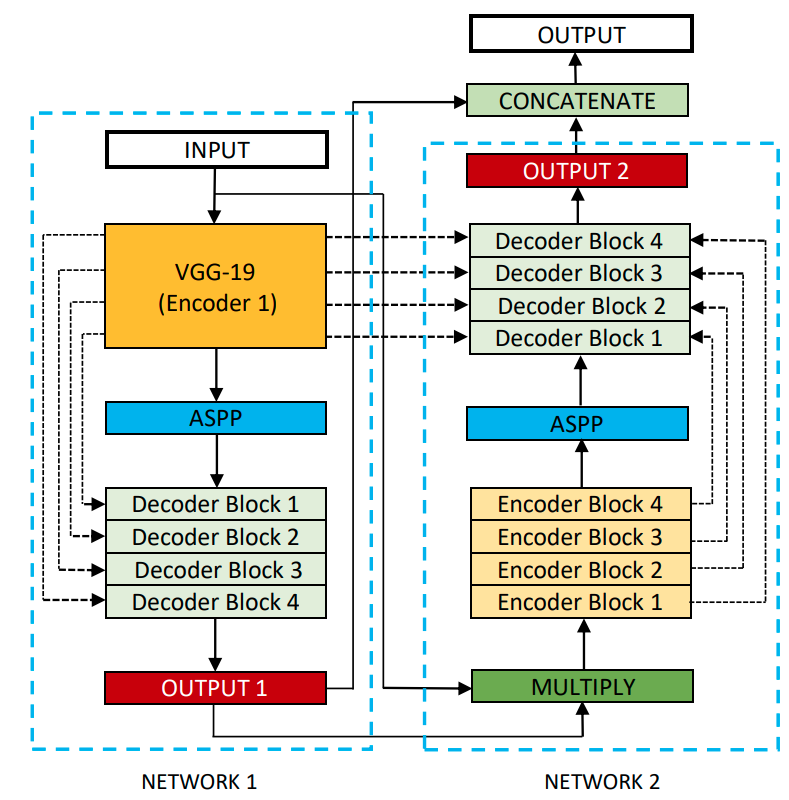
\includegraphics[width=\textwidth]{images/double_unet.png}
\captionof{figure}{Double U-Net model \cite{DOUBLE_UNET:2020}}
\end{center}
% TODO: Double U-Net
% -> PyEDDL
% -> Tensorflow
%
% -> Dice scores
% -> Profiles
% -> Network output

\newpage
\subsection{Double U-Net evaluation}

\begin{figure*}[!htb]
    \subfigure[tr943]{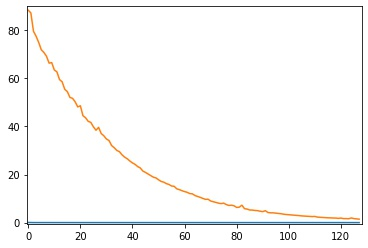
\includegraphics[width=.47\textwidth]{images/aux.jpg}\label{fig:tr943}}\hfill
    \subfigure[tr1426]{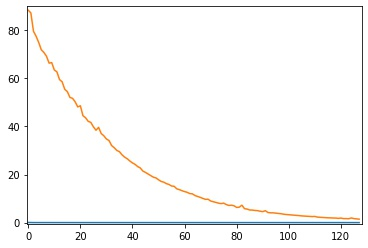
\includegraphics[width=.47\textwidth]{images/aux.jpg}\label{fig:tr1426}}
    
    \subfigure[tr943]{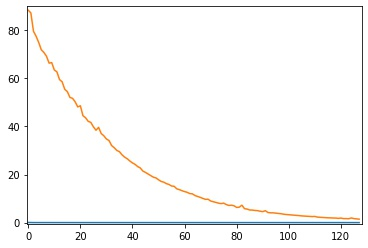
\includegraphics[width=.47\textwidth]{images/aux.jpg}\label{fig:tr943}}\hfill
    \subfigure[tr1426]{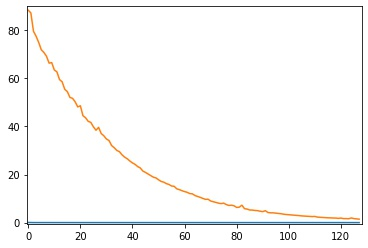
\includegraphics[width=.47\textwidth]{images/aux.jpg}\label{fig:tr1426}}
    
    \subfigure[tr943]{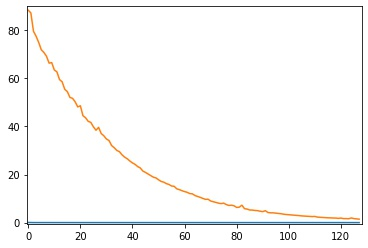
\includegraphics[width=.47\textwidth]{images/aux.jpg}\label{fig:tr943}}\hfill
    \subfigure[tr1426]{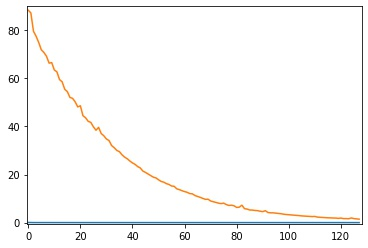
\includegraphics[width=.47\textwidth]{images/aux.jpg}\label{fig:tr1426}}

    \subfigure[tr943]{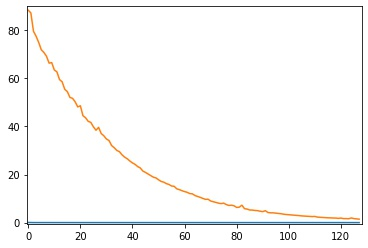
\includegraphics[width=.47\textwidth]{images/aux.jpg}\label{fig:tr943}}\hfill
    \subfigure[tr1426]{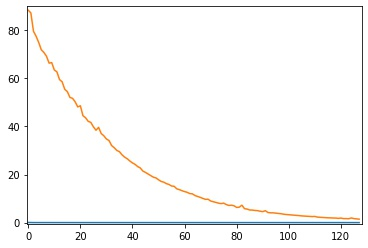
\includegraphics[width=.47\textwidth]{images/aux.jpg}\label{fig:tr1426}}
\end{figure*}

\newpage
\subsection{Double U-Net profiling}

\begin{figure*}[!htb]
    \subfigure[tr943]{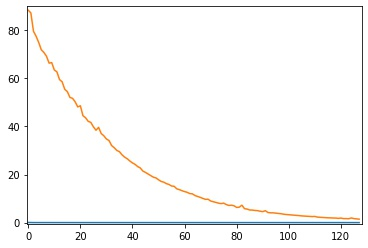
\includegraphics[width=.47\textwidth]{images/aux.jpg}\label{fig:tr943}}\hfill
    \subfigure[tr1426]{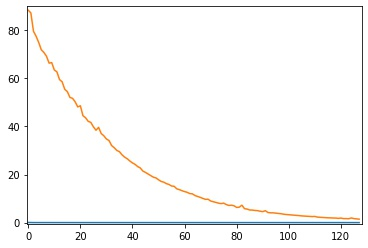
\includegraphics[width=.47\textwidth]{images/aux.jpg}\label{fig:tr1426}}
    
    \subfigure[tr943]{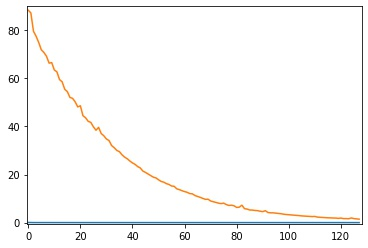
\includegraphics[width=.47\textwidth]{images/aux.jpg}\label{fig:tr943}}\hfill
    \subfigure[tr1426]{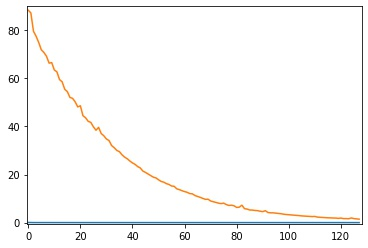
\includegraphics[width=.47\textwidth]{images/aux.jpg}\label{fig:tr1426}}
    
    \subfigure[tr943]{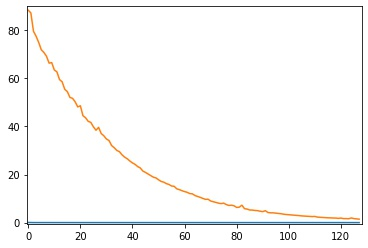
\includegraphics[width=.47\textwidth]{images/aux.jpg}\label{fig:tr943}}\hfill
    \subfigure[tr1426]{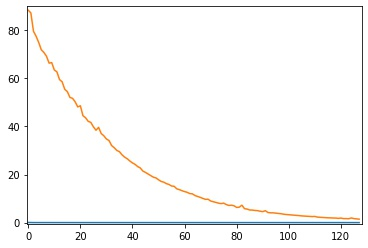
\includegraphics[width=.47\textwidth]{images/aux.jpg}\label{fig:tr1426}}

    \subfigure[tr943]{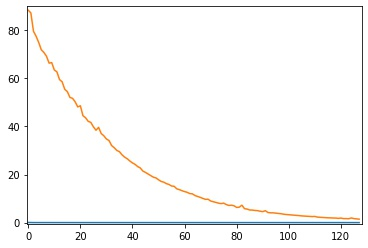
\includegraphics[width=.47\textwidth]{images/aux.jpg}\label{fig:tr943}}\hfill
    \subfigure[tr1426]{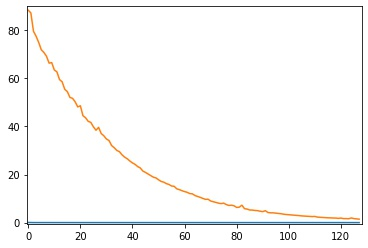
\includegraphics[width=.47\textwidth]{images/aux.jpg}\label{fig:tr1426}}
\end{figure*}



%%%%%%% COMPARISON
\newpage
\section{Comparison}

